\paragraph{Monkeys exhibit biases} %hallmarks of color category behavior

The animals examined show a hallmark of color categorization behavior: memory biases towards a set of particular points in a perceptually uniform colorspace.
In \autoref{fig:AvResults} it can be seen that the biases deviate substantially and systematically from zero, with the attractor points being found where the bias line crosses the zero line from positive to negative (going counter-clockwise). These points are highlighted with colored lines, with the filled areas around these lines showing the confidence intervals on these crossing points. Repeller points found where the line crosses the zero line from negative to positive.



\paragraph{Shared color categories across monkeys}

We see that all tested monkeys share two common attractor points (\autoref{fig:BiasCurvesIndividual}), which we interpret as evidence of two shared color categories: a warm/orange-ish category (between 0$^\circ$ and 45$^\circ$), and a cool/blue-ish category (between 180$^\circ$ and 225$^\circ$). 

% Results table?

%\begin{figure}
%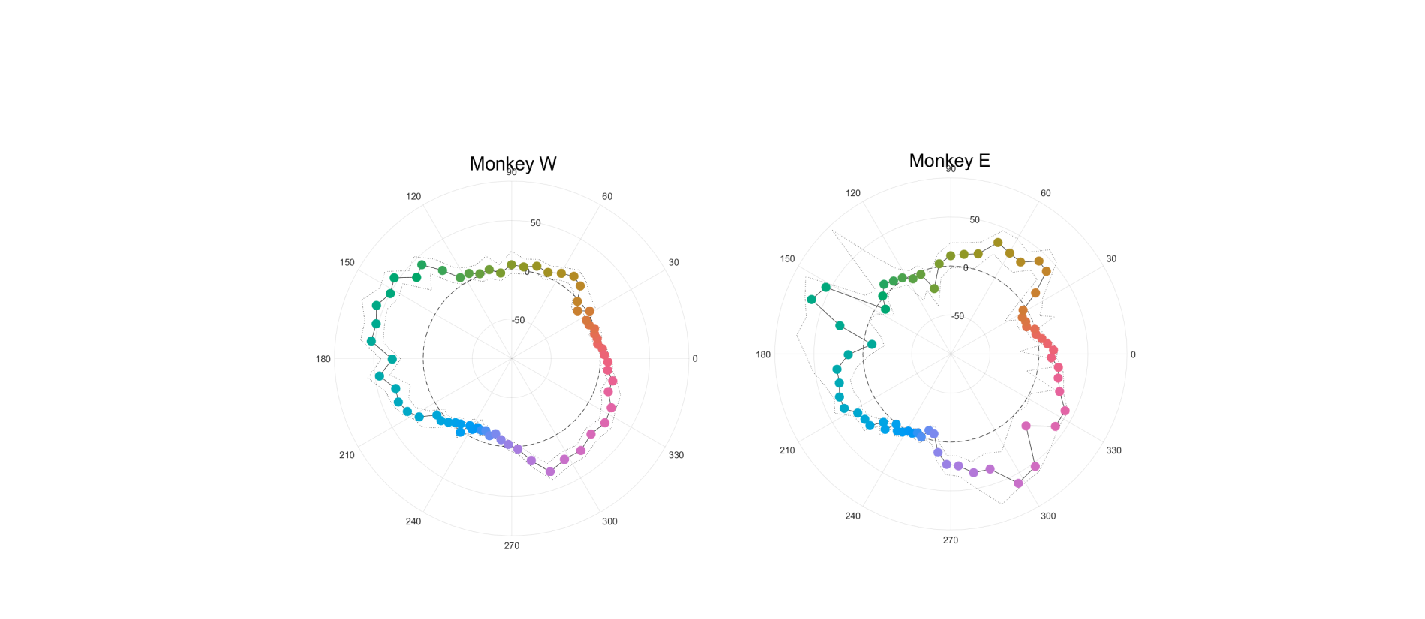
\includegraphics[width=\textwidth]{../../Figures/Old/panichellobias.pdf}
%\caption{Bias as a function of hue, for Panichello monkeys} 
%\end{figure}

\paragraph{Biases Compared to Humans}

Comparison to our human data, Mech Turk and also rig (maybe?)

Comparison to \cite{bae_why_2015}

Comparison to \cite{panichello_error-correcting_2019}

\paragraph{Cognitive Bias vs. Non-uniformity in Perceptual Space}



\paragraph{A behaviorally-derived colorspace}

Extracted colorspace shown in \autoref{fig:MACBEHcolorspace}.

\paragraph{Individual differences between monkeys}

In one animal \autoref{fig:BiasCurvesCastor} we see evidence of additional categories: strong evidence for a greenish category and weak evidence for a purple category (the ``strength" of a category can be gleaned from looking at the local gradient at the zero-crossing point)

\begin{figure}
\includesvg[pretex=\tiny, width=\textwidth]{../Figures/working/6_IndiData_CogBias/sm_18_230708-094920.svg}
\caption{\textbf{Lorem.}
Ipsum.
}
\label{fig:IndiDataCogBias}
\end{figure}